\chapter{Priority First Search}
\label{chap:priorityfirst}

De laatste methode die onderzocht is, is Dijkstra's algoritme. Dit algoritme geeft prioriteiten aan de knopen en gaat aan de hand hiervan de knopen bijlangs.

De methode verwacht als invoer een graaf $g$, een startknoop $s$ en een eindknoop $t$.
Als eerste wordt de maxflow van alle knopen in $g$ op 0 gezet, behalve de maxflow van $s$, deze krijgt de waarde \infty. Al deze knopen worden toegevoegt aan een priorityqueue $Q$, de maxflow van de knopen wordt gebruikt als de prioriteit.
Nu zal het algoritme doorgaan tot $Q$ leeg is. Elke keer zal de hoogste waarde in $Q$ verwijderd worden, deze waarde krijgt hier de naam $u$. De eerste keer zal dit $s$ zijn. Elke keer wanneer een knoop $u$ uit $Q$ gehaald wordt zullen alle kanten van $u$ bezocht worden. Voor elke kant zal de overstaande knoop ($z$) van $u$ via kant $e$ opgezocht worden. De flow die naar $z$ kan is de maxflow van $u$ of de residual capacity van $e$ als deze lager is dan de maxflow van $u$. Wanneer de flow van $u$ naar $z$ hoger is dan de huidige maxflow van $z$, zal deze bijgewerkt worden. Nu zal ook de waarde van $z$ in $Q$ geupdate worden.

\subsection{Pseudocode}
De pseudocode waar de code op gebaseerd is is te vinden in algoritme \ref{alg:DIJKSTRA}.
De werkelijke code heeft een paar toevoegingen zodat deze stopt wanneer het eindpunt $t$ bereikt is. Wanneer dit het geval is kan met behulp van de $parents$ gezocht worden naar een pad van $s$ naar $t$ door te kijken wat de parent edge $e$ is van $t$. Nu zal gekeken worden naar de parent edge van de overstaande van $t$ via edge $e$. Door dit te doen tot er geen parent edge is zal $s$ bereikt worden.

\begin{algorithm}[h]
\caption{Dijkstra's Algorithm}
\label{alg:DIJKSTRA}
\begin{algorithmic}
\REQUIRE Input: Graph g, Start vertex s, End vertex t
\STATE HashMap parents with vertexes and edges
\STATE Q $\gets$ new PriorityQueue
\FORALL{vertex $v \in g.vertexes$}
\IF{$v = s$}
\STATE $v.maxFlow \gets \infty$
\ELSE
\STATE $v.maxFlow \gets 0$
\ENDIF
\STATE Q.add(maxFlow, v)
\STATE set parent to \emptyset
\ENDFOR
\WHILE{Q is not empty}
\STATE $u \gets Q.removeMax()$
\FORALL{edge $e \in u.incidentEdges$}
\STATE $z \gets g.opposite(u, e)$
\STATE $r \gets min(u.getResidualCapacity(e), u.maxFlow)$
\IF{$r < z.maxFlow && e \neg= parent of z$}
\STATE $z.maxFlow \gets r$
\STATE set $e$ as parent of $z$
\STATE update $z$ in $Q$
\ENDIF
\ENDFOR
\ENDWHILE
\end{algorithmic}
\end{algorithm}

\subsection{Analyse}

Figuur \ref{fig:DIJKSTRA_graph1} en \ref{fig:DIJKSTRA_graph2} laten de uitkomst zien van de analyse.

\begin{figure}[h]
	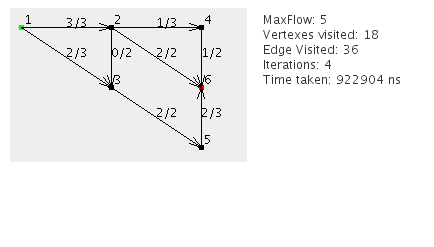
\includegraphics[width=0.5\linewidth]{depthfirst/DIJKSTRA_graph1}
	\centering
	\caption{Analyse van de eerste graaf}
	\label{fig:DIJKSTRA_graph1}
\end{figure}

\begin{figure}[h]
	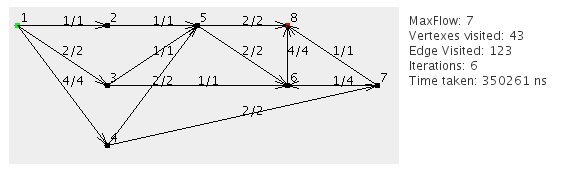
\includegraphics[width=0.5\linewidth]{depthfirst/DIJKSTRA_graph2}
	\centering
	\caption{Analyse van de tweede graaf}
	\label{fig:DIJKSTRA_graph2}
\end{figure}